\documentclass[a4paper,11pt]{article}

\usepackage[utf8]{inputenc}
\usepackage[T1]{fontenc}
\usepackage{amsmath, amssymb, amsfonts, amsthm}
\usepackage{graphicx}
\usepackage{hyperref}
\usepackage{geometry}
\usepackage{booktabs}
\usepackage{float}
\usepackage{subcaption}
\usepackage{fancyhdr}
\usepackage{xcolor}
\usepackage{listings}
\usepackage{array}
\usepackage{multirow}
\usepackage{colortbl}
\usepackage{tikz}
\usepackage{pgfplots}
\pgfplotsset{compat=1.18}

\definecolor{okgreen}{RGB}{34,139,34}
\definecolor{alertred}{RGB}{180,30,30}
\definecolor{codeblue}{RGB}{30,80,160}
\definecolor{codegray}{RGB}{120,120,120}
\definecolor{codelightgray}{RGB}{248,248,248}

\lstset{
  language=Python,
  basicstyle=\small\ttfamily,
  keywordstyle=\color{codeblue}\bfseries,
  commentstyle=\color{codegray}\itshape,
  stringstyle=\color{okgreen},
  frame=single,
  backgroundcolor=\color{codelightgray},
  breaklines=true,
  numbers=left,
  numberstyle=\tiny\color{codegray},
  xleftmargin=1.5em,
  showstringspaces=false
}

\pagestyle{fancy}
\renewcommand{\headrulewidth}{0pt}
\fancyhead[C]{%
    \makebox[\textwidth][c]{Data Battle 2026 --- Rapport final de modélisation}\\
    \makebox[\textwidth][c]{\rule{0.9\textwidth}{0.1pt}}
}
\fancyhead[L]{}\fancyhead[R]{}
\fancyfoot[L]{}\fancyfoot[R]{}
\fancyfoot[C]{\makebox[\textwidth][c]{\thepage}}
\setlength{\headheight}{25pt}

\geometry{hmargin=2cm,vmargin=2.5cm}

\newtheorem{definition}{Definition}[section]
\newtheorem{proposition}{Proposition}[section]
\newtheorem{theoreme}{Theoreme}[section]
\newtheorem{remarque}{Remarque}[section]

\title{%
  \textbf{Prediction probabiliste de la fin d'alerte foudre}\\[0.4em]
  \large Processus de Hawkes, LightGBM et quantile regression\\
  \large pour l'estimation du delai optimal de levee d'alerte
}
\author{ZEROUALI Mohammed Amine \& BOUBEKRI Saad}
\date{\textit{Data Battle 2026 --- Meteorage}}

\begin{document}
\maketitle

\begin{abstract}
Ce rapport presente la solution complete developpee pour le Data Battle 2026 de
Meteorage. Le probleme consiste a estimer, en temps reel, le moment auquel une
alerte foudre autour d'un aeroport peut etre levee en toute securite --- en
gagnant du temps par rapport a la methode reglementaire fixe de 30 minutes.
Deux approches complementaires sont developpees : un processus de Hawkes
auto-excitant pour la modelisation probabiliste rigoureuse, et un modele
LightGBM avec quantile regression pour la prediction supervisee. L'approche
hybride combine les deux en utilisant l'intensite de Hawkes comme feature
d'entree du gradient boosting. Les resultats obtenus sur le jeu d'evaluation
du jury montrent un \textbf{gain total de 80 heures} sur 412 alertes, avec un
risque maitrise $R = 1.82\% < 2\%$ au seuil optimal $\theta^* = 0.85$, et
une calibration des quantiles validee experimentalement.
\end{abstract}

\tableofcontents
\newpage

%=============================================================
\section{Problematique et donnees}
%=============================================================

\subsection{Contexte metier}

Un aeroport doit suspendre certaines activites au sol des qu'un impact de foudre
survient dans un rayon de 20 km. La methode actuelle maintient l'alerte active
pendant \textbf{30 minutes fixes} apres le dernier impact observe, quelle que
soit la dynamique reelle de l'orage. Cette approche conservative est sure mais
penalisante : pour un orage qui s'eloigne rapidement, on attend inutilement.

L'objectif est de produire, a chaque instant $\tau_n$ d'une alerte en cours,
une \textbf{prediction de la fin reelle de l'alerte} avec un niveau de confiance
quantifie --- permettant une reprise d'activite jusqu'a 15--20 minutes plus tot
tout en maintenant un risque de foudre manquee inferieur a 2\%.

\subsection{Donnees fournies par Meteorage}

Les donnees contiennent $\sim$507\,000 impacts de foudre sur 10 ans
(2016--2025), georeferencies et horodates autour de 6 aeroports europeens.

\begin{table}[H]
\centering
\begin{tabular}{lcccc}
\toprule
Colonne & Type & Description \\
\midrule
\texttt{date} & datetime UTC & Instant de l'impact \\
\texttt{lon}, \texttt{lat} & float & Position geographique (WGS84) \\
\texttt{amplitude} & float (kA) & Intensite du courant de decharge \\
\texttt{dist} & float (km) & Distance a l'aeroport \\
\texttt{icloud} & bool & Nuage-sol (False) ou intra-nuageux (True) \\
\texttt{airport\_alert\_id} & float & Identifiant de l'alerte (si dist $\leq 20$ km) \\
\texttt{is\_last\_lightning\_cloud\_ground} & bool & Dernier eclair sol de l'alerte \\
\bottomrule
\end{tabular}
\caption{Description des colonnes du fichier de donnees brutes.}
\end{table}

\begin{table}[H]
\centering
\begin{tabular}{lcccc}
\toprule
Aeroport & Alertes (train) & Impacts (train) & Alertes (eval) & Position \\
\midrule
Ajaccio  & 407 & 15\,321 & 96  & lon=8.80,  lat=41.92 \\
Bastia   & 424 & 21\,738 & 141 & lon=9.48,  lat=42.55 \\
Biarritz & 486 & 23\,669 & 118 & lon=-1.52, lat=43.47 \\
Nantes   & 173 & 8\,410  & 45  & lon=-1.61, lat=47.15 \\
Pise     & 623 & 29\,174 & 146 & lon=10.40, lat=43.70 \\
\midrule
\textbf{Total} & \textbf{2\,113} & \textbf{98\,312} & \textbf{546} & \\
\bottomrule
\end{tabular}
\caption{Repartition des alertes par aeroport apres pretraitement.}
\end{table}

%=============================================================
\section{Pretraitement et nettoyage des donnees}
%=============================================================

\subsection{Definition operationnelle d'une alerte}

\begin{definition}[Alerte foudre]
Une alerte est declenchee a l'instant $\tau_0$ lors du premier impact dans le
disque $\mathcal{D} = B(A, 20\text{ km})$ centre sur l'aeroport $A$. Elle se
termine a la premiere periode de $\Delta = 30$ minutes consecutives sans impact
dans $\mathcal{D}$.
\end{definition}

\subsection{Probleme des multi-detections}

\textbf{Observation critique.} Plusieurs lignes du fichier partagent le meme
timestamp pour le meme aeroport : c'est le meme eclair physique detecte
simultanement par plusieurs capteurs du reseau Meteorage. Ces doublons
faussent l'estimation des parametres si on ne les traite pas.

\textbf{Diagnostic quantitatif.} Sans deduplication, le MLE du processus de
Hawkes estimait $\hat\alpha \approx 254$ impacts/min (physiquement absurde).
Apres deduplication a 10 secondes : $\hat\alpha \approx 0.21$ impacts/min
(coherent avec la physique orageuse).

\begin{table}[H]
\centering
\begin{tabular}{lccc}
\toprule
Seuil de deduplication & $\hat\alpha$ (Ajaccio) & Duree simulee moy. & Physique ? \\
\midrule
Aucune & 254.1 & $\gg 6$h & Non \\
10 secondes & 0.212 & $\sim 40$--80 min & Oui \\
1 minute & 0.049 & $\sim 200$ min & Non \\
\bottomrule
\end{tabular}
\caption{Impact du seuil de deduplication sur les parametres estimes.}
\end{table}

\textbf{Choix retenu : 10 secondes.} Ce seuil elimine les multi-detections
(separees de $<1$ s) tout en conservant les impacts physiquement distincts.

\subsection{Gestion des identifiants d'alerte dans les donnees de test}

\textbf{Difficulte specifique au jeu de test.} Le fichier de test fourni par le
jury contient une colonne \texttt{airport\_alert\_id} majoritairement vide
(\texttt{NaN}) : seuls les impacts correspondant aux alertes de reference sont
labellises. Un \texttt{groupby('airport\_alert\_id')} classique ignore
silencieusement les \texttt{NaN}, ce qui ferait perdre les alertes non encore
labellisees.

\textbf{Solution retenue.} La segmentation est effectuee par \textbf{silence de
30 minutes} (identique au pipeline d'entrainement), puis l'identifiant
\texttt{airport\_alert\_id} est recupere comme premiere valeur non-\texttt{NaN}
dans chaque segment. Cette approche garantit que toutes les alertes reelles
sont traitees, qu'elles soient labellisees ou non.

\subsection{Pipeline de pretraitement}

\begin{enumerate}
  \item Parsing des dates en UTC, conversion en minutes depuis l'epoque Unix.
  \item Filtrage : $\texttt{dist} \leq 20$ km (zone alerte) et
        $\texttt{dist} \leq 50$ km (zone etendue pour features spatiales).
  \item Deduplication a 10 secondes par aeroport.
  \item Segmentation en alertes par silence de 30 minutes.
  \item Stockage des timestamps relatifs (depuis $\tau_0 = 0$) et absolus en
        parallele pour permettre la reconstruction des features spatiales.
\end{enumerate}

\begin{lstlisting}
# Conversion correcte pour timestamps timezone-aware
df['t_min'] = (df['date'] - pd.Timestamp('1970-01-01', tz='UTC')
               ).dt.total_seconds() / 60

# Deduplication a 10 secondes
GAP_DEDUP = 10 / 60   # minutes
keep = [0]
for i in range(1, len(t_abs)):
    if t_abs[i] - t_abs[keep[-1]] >= GAP_DEDUP:
        keep.append(i)
\end{lstlisting}

\textbf{Note technique.} L'utilisation de \texttt{.values.astype('int64') / 1e9}
pour les timestamps timezone-aware produit des valeurs erronees (1970 au lieu
de 2023). La soustraction directe avec \texttt{pd.Timestamp('1970-01-01',
tz='UTC')} est la seule methode fiable.

%=============================================================
\section{Formulation mathematique du probleme}
%=============================================================

\subsection{Modele probabiliste}

On se place sur un espace de probabilite filtre
$(\Omega, \mathcal{F}, (\mathcal{F}_t)_{t\geq 0}, \mathbb{P})$. Les impacts
dans $\mathcal{D}$ sont modelises par un \textbf{processus ponctuel marque} :
\[
\mathcal{N} = \{(\tau_i, \mathbf{X}_i)\}_{i \geq 1}
\]
ou $\tau_i \in \mathbb{R}_+$ est l'instant d'impact et
$\mathbf{X}_i = (\xi_i, \phi_i, \alpha_i, d_i, C_i)$ le vecteur de marques
(position, amplitude, distance, type).

\subsection{Objectif probabiliste}

A l'instant $\tau_n$ du dernier impact observe, avec historique
$\mathcal{H}_n = \sigma(\tau_i, \mathbf{X}_i \mid 0 \leq i \leq n)$, on
cherche le \textbf{delai minimal de levee d'alerte} :

\[
\boxed{u^* = \inf\left\{u \in [0, \Delta] \;\middle|\;
\mathbb{P}(T > \tau_n + u \mid \mathcal{H}_n) < \varepsilon \right\}}
\]

ou $T$ est la duree totale de l'alerte et $\varepsilon$ le risque tolere.

\subsection{Criteres d'evaluation du jury}

Le jury evalue les predictions selon deux criteres combines.

\textbf{Gain de temps.} Pour une prediction $\hat{t}^a$ de fin d'alerte $a$ :
\[
g^a = t^a + 30 - \hat{t}^a
\]
ou $t^a$ est le timestamp du dernier vrai eclair. Le gain global est
$G = \sum_a g^a$.

\textbf{Risque.} Proportion d'eclairs dangereux (dist $< 3$ km) survenant
\emph{apres} la fin d'alerte predite :
\[
R = \frac{M^{L3}}{N^{L3}}, \quad
M^{L3} = \sum_i \mathbf{1}_{d_i < 3 \;\&\; \hat{t}^a < t_i \;\&\; \text{alert}(t_i) = a}
\]

\textbf{Selection du seuil.} Le jury balaye $\theta \in [0, 1]$. Pour chaque
$\theta$, la prediction retenue par alerte est :
\[
\hat{t}^a = \min_i \hat{t}^a_i, \quad s^a_i \geq \theta
\]
Le $\theta^*$ optimal maximise $G$ sous la contrainte $R < R_{\text{accept}} =
0.02$.

\textbf{Lien avec notre modele.} Notre confiance $s = 1 - \varepsilon$ est le
complement du risque tolere. Plus $\varepsilon$ est petit, plus la prediction
est conservative (confiance elevee, gain faible). Le balayage de $\theta$
correspond exactement au balayage de $\varepsilon$ dans notre modele.

%=============================================================
\section{Approche 1 : Processus de Hawkes}
%=============================================================

\subsection{Choix du modele}

\begin{definition}[Processus de Hawkes a noyau exponentiel]
L'intensite conditionnelle est :
\[
\lambda^*(t) = \mu + \alpha \sum_{\tau_i < t} e^{-\beta(t - \tau_i)}
\]
avec $\mu > 0$ (taux de fond), $\alpha > 0$ (excitabilite), $\beta > 0$
(decroissance). La stationnarite exige $\alpha/\beta < 1$.
\end{definition}

\textbf{Justification physique.} Chaque impact ionise localement l'atmosphere,
augmentant la probabilite d'impacts suivants dans les minutes qui suivent. La
memoire exponentielle decroissante capture ce phenomene d'auto-excitation a
courte portee temporelle.

\subsection{Variable recursive et calcul en O(n)}

La variable recursive $R_i = \sum_{j < i} e^{-\beta(\tau_i - \tau_j)}$ se met
a jour en $O(1)$ :
\[
R_i = e^{-\beta(\tau_i - \tau_{i-1})}(1 + R_{i-1}), \quad R_0 = 0.
\]
L'intensite en $\tau_i$ est alors $\lambda^*(\tau_i) = \mu + \alpha R_i$.

\subsection{Estimation par maximum de vraisemblance}

Pour une trajectoire $\{\tau_0, \ldots, \tau_n\}$ observee sur $[0, T_k]$
avec $T_k = \tau_n + \Delta$ :
\[
\ell_k(\mu, \alpha, \beta) =
\sum_{i=0}^{n} \log(\mu + \alpha R_i)
- \mu T_k - \frac{\alpha}{\beta}\sum_{i=0}^{n}\left(1 - e^{-\beta(T_k - \tau_i)}\right).
\]

La log-vraisemblance totale $\mathcal{L} = \sum_k \ell_k$ est maximisee par
L-BFGS-B avec une grille d'initialisations.

\subsection{Resultats de l'estimation}

\begin{table}[H]
\centering
\begin{tabular}{lcccc}
\toprule
Aeroport & $\hat\mu$ (imp/min) & $\hat\alpha$ & $\hat\beta$ (min$^{-1}$) &
$\hat\alpha/\hat\beta$ \\
\midrule
Ajaccio  & 0.0557 & 0.212 & 0.241 & 0.880 \\
Bastia   & 0.0561 & 0.215 & 0.237 & 0.904 \\
Biarritz & 0.0540 & 0.231 & 0.253 & 0.914 \\
Nantes   & 0.0574 & 0.231 & 0.256 & 0.903 \\
Pise     & 0.0562 & 0.204 & 0.229 & 0.892 \\
\bottomrule
\end{tabular}
\caption{Parametres du processus de Hawkes estimes par MLE (unites : minutes).
$1/\hat\beta \approx 4$ min : duree caracteristique de l'excitation.
$\hat\alpha/\hat\beta \approx 0.9$ : processus sous-critique, stationnaire.}
\end{table}

\subsection{Validation : theoreme de rescaling temporel}

\begin{theoreme}[Papangelou, 1972]
Si le modele est correctement specifie, les accroissements de la compensatrice
$U_i = \Lambda(\tau_i) - \Lambda(\tau_{i-1})$ sont i.i.d. $\sim \mathrm{Exp}(1)$.
\end{theoreme}

Le test de Kolmogorov-Smirnov est rejete pour tous les aeroports
(stat. KS $\approx$ 0.28--0.38, $p < 0.001$), ce qui revele une
\textbf{inadequation structurelle} du modele stationnaire.

\subsection{Diagnostic de l'inadequation}

Avec $\hat\mu \approx 0.056$ imp/min :
\[
P(\text{silence de 30 min}) = e^{-\hat\mu \times 30} = e^{-1.68} \approx 18.7\%,
\]
soit une duree simulee moyenne $\approx 30/0.187 \approx 160$ min alors que les
alertes reelles durent 60--140 min.

\textbf{Cause fondamentale.} Le Hawkes \emph{stationnaire} suppose $\mu =
\text{const}$. Or les orages sont des \textbf{phenomenes spatialement mobiles}
a duree de vie finie : ils entrent dans le disque, y restent, puis le quittent.
L'intensite reelle forme une cloche temporelle que $\mu$ constant ne peut pas
representer.

\textbf{Ce que le Hawkes apporte malgre cette limite.} L'intensite courante
$\lambda^*(\tau_n)$ est une \textbf{feature hybride} tres informative : une
valeur elevee signifie que l'orage est actif, une valeur faible signifie qu'il
se calme. C'est l'un des top 2 features du modele LightGBM.

%=============================================================
\section{Approche 2 : LightGBM avec quantile regression}
%=============================================================

\subsection{Reformulation comme probleme supervise}

A chaque instant $\tau_n$ au sein d'une alerte, on predit la variable :
\[
y = \tau_{n+1} - \tau_n \in (0, 30] \text{ minutes}
\]
c'est-a-dire le \textbf{delai avant le prochain impact} (ou 30 min si $\tau_n$
est le dernier impact de l'alerte). Cette cible est directement liee a $u^*$ :
si le modele predit $\hat{y} = 25$ min, l'alerte ne se terminera probablement
pas avant 25 min.

\subsection{Pourquoi LightGBM}

LightGBM est un algorithme de gradient boosting sur arbres de decision :
\[
F(\mathbf{f}) = \sum_{m=1}^{M} \eta \cdot h_m(\mathbf{f}),
\]
ou chaque arbre $h_m$ corrige les erreurs residuelles du precedent. Sa
construction feuille par feuille (\emph{leaf-wise}) lui permet de capturer des
interactions non lineaires complexes entre features sans hypothese
distributionnelle.

\textbf{Avantages cles pour ce probleme :}
\begin{itemize}
  \item Aucune hypothese sur la forme de l'intensite $\lambda^*(t)$ --- pas de
        contrainte de stationnarite
  \item Integration naturelle des marques (amplitude, distance, type d'eclair)
  \item Support natif de la \textbf{quantile regression} --- permet de produire
        une distribution complete plutot qu'une seule valeur
  \item Rapide a l'entrainement : 92\,377 exemples en $< 5$ min CPU
\end{itemize}

\subsection{Construction des features}

Pour chaque instant de prediction $\tau_n$, le vecteur de features
$\mathbf{f}_n \in \mathbb{R}^{12}$ est :

\begin{table}[H]
\centering
\renewcommand{\arraystretch}{1.3}
\begin{tabular}{p{3.5cm} p{6cm} p{3.5cm}}
\toprule
Feature & Description & Justification \\
\midrule
\texttt{duree\_ecoulee} & $\tau_n$ depuis le debut de l'alerte (min) &
  \textbf{Top 1} : un orage long a tendance a se terminer \\
\texttt{lambda\_hawkes} & $\lambda^*(\tau_n) = \mu + \alpha R_n$ &
  \textbf{Top 2} : mesure l'excitation courante \\
\texttt{ia\_last} & $\tau_n - \tau_{n-1}$ (min) &
  \textbf{Top 3} : trend direct de ralentissement \\
\texttt{amp\_last} & $|\alpha_n|$ kA &
  Top 4 : amplitude du dernier eclair \\
\texttt{n\_impacts} & Nombre d'impacts depuis $\tau_0$ &
  Top 5 : intensite totale de l'orage \\
\texttt{amp\_mean} & Amplitude moyenne sur l'alerte &
  Signature de l'intensite orageuse \\
\texttt{ia\_mean3}, \texttt{ia\_mean5} & Moyenne des 3, 5 dernieres inter-arrivees &
  Tendance de ralentissement \\
\texttt{prop\_cloud} & Proportion d'eclairs intra-nuageux &
  Signature du type d'orage \\
\texttt{ia\_max}, \texttt{ia\_min} & Extremes des inter-arrivees &
  Amplitude de la dynamique \\
\texttt{ia\_slope} & Pente des dernieres inter-arrivees &
  Acceleration ou ralentissement \\
\bottomrule
\end{tabular}
\caption{Features du modele LightGBM par ordre d'importance decroissant.}
\label{tab:features}
\end{table}

\subsection{Quantile regression : pourquoi et comment}

Au lieu de predire $\mathbb{E}[y \mid \mathbf{f}_n]$ (mediane), on entraine
\textbf{13 modeles} independants, un par quantile
$q \in \{0.05, 0.10, 0.15, 0.20, 0.30, 0.40, 0.50, 0.60, 0.70, 0.80, 0.85,
0.90, 0.95\}$.

Chaque modele minimise la \textbf{pinball loss} :
\[
\rho_q(r) = r \cdot (q - \mathbf{1}_{r < 0}), \quad r = y - \hat{y}_q.
\]

Les 13 quantiles estimes $\hat{Q}_q(y \mid \mathbf{f}_n)$ approximent la
\textbf{fonction de repartition conditionnelle} $F_{Y|\mathbf{f}_n}$. La
courbe de survie est alors :
\[
\hat{S}(u) = \mathbb{P}(y > u \mid \mathbf{f}_n) = 1 - \hat{F}_{Y|\mathbf{f}_n}(u)
\approx 1 - \text{interp}(u,\, \hat{Q}_{0.05}, \ldots, \hat{Q}_{0.95})
\]
et le delai optimal :
\[
u^* = \inf\{u \in [0, 30] \mid \hat{S}(u) < \varepsilon\}.
\]

\subsection{Calibration des quantiles}

Un modele de quantile est bien calibre si la couverture reelle est proche du
quantile theorique, i.e. $\mathbb{P}(y \leq \hat{Q}_q) \approx q$.

\begin{table}[H]
\centering
\begin{tabular}{ccc}
\toprule
Quantile $q$ & Couverture reelle & Ecart \\
\midrule
0.05 & 0.075 & +0.025 \\
0.10 & 0.124 & +0.024 \\
0.50 & 0.498 & $-0.002$ \\
0.70 & 0.729 & +0.029 \\
0.80 & 0.799 & $-0.001$ \\
0.90 & 0.894 & $-0.006$ \\
0.95 & 1.000 & +0.050 \\
\bottomrule
\end{tabular}
\caption{Calibration des quantiles sur le jeu de validation (split 80/20).
Les quantiles mediocres aux extremes (0.05, 0.95) sont classiques sur un
petit dataset et n'affectent pas $u^*$ calcule pour $\varepsilon = 0.10$--$0.20$.}
\end{table}

\subsection{Resultats finaux sur le jeu d'evaluation}

\begin{table}[H]
\centering
\renewcommand{\arraystretch}{1.3}
\begin{tabular}{lc}
\toprule
Metrique & Valeur \\
\midrule
Seuil optimal $\theta^*$ & 0.85 \\
Risque $R$ (metrique jury) & 1.82\% $< 2\%$ \checkmark \\
Gain total & 80 heures \\
Alertes couvertes & 412 / 612 \\
Predictions generees & 323\,820 lignes \\
Entrainement (92\,377 exemples, 13 modeles) & $< 5$ min CPU \\
\bottomrule
\end{tabular}
\caption{Resultats du modele sur le jeu d'evaluation du jury (612 alertes, 5 aeroports).}
\end{table}

\begin{table}[H]
\centering
\renewcommand{\arraystretch}{1.3}
\begin{tabular}{lrrc}
\toprule
Aeroport & Alertes couvertes & Gain (h) & Eclairs manques \\
\midrule
Ajaccio  & 96  & 25.5 & 2 \\
Bastia   & 141 & 20.3 & 5 \\
Biarritz & 118 &  7.8 & 0 \\
Nantes   &  45 &  5.7 & 0 \\
Pise     & 146 & 21.3 & 0 \\
\midrule
\textbf{Total} & \textbf{546} & \textbf{80.6} & \textbf{7} \\
\bottomrule
\end{tabular}
\caption{Detail par aeroport a $\theta^* = 0.85$.
Les 7 eclairs manques (sur 385 eclairs dangereux totaux) correspondent a $R = 1.82\%$.}
\end{table}

%=============================================================
\section{Pipeline de generation des predictions}
%=============================================================

\subsection{Vue d'ensemble}

\begin{center}
\begin{tikzpicture}[
  box/.style={rectangle, rounded corners=6pt, draw=gray, fill=gray!10,
              minimum width=4.5cm, minimum height=0.9cm,
              text centered, font=\small},
  arr/.style={->, thick, gray}
]
\node[box] (A) at (0,0)    {Donnees train brutes};
\node[box] (B) at (0,-1.5) {Pretraitement + dedup};
\node[box] (C) at (0,-3.0) {MLE Hawkes par aeroport};
\node[box] (D) at (0,-4.5) {Construction features (92\,377 lignes)};
\node[box] (E) at (0,-6.0) {Entrainement 13 modeles LightGBM};
\node[box] (F) at (0,-7.5) {Donnees test tronquees};
\node[box] (G) at (0,-9.0) {Prediction $u^*(\varepsilon)$ x 9 niveaux};
\node[box] (H) at (0,-10.5){predictions.csv (323\,820 lignes)};

\draw[arr] (A) -- (B);
\draw[arr] (B) -- (C);
\draw[arr] (C) -- (D);
\draw[arr] (D) -- (E);
\draw[arr] (E) -- (G);
\draw[arr] (F) -- (G);
\draw[arr] (G) -- (H);
\end{tikzpicture}
\end{center}

\subsection{Format du fichier predictions.csv}

Conforme au format attendu par le jury :

\begin{table}[H]
\centering
\begin{tabular}{lll}
\toprule
Colonne & Type & Description \\
\midrule
\texttt{airport} & str & Nom de l'aeroport \\
\texttt{airport\_alert\_id} & float & ID de l'alerte (fourni par le jury) \\
\texttt{prediction\_date} & datetime UTC & Timestamp de $\tau_n$ (instant de prediction) \\
\texttt{predicted\_date\_end\_alert} & datetime UTC & Timestamp de $\tau_n + u^*(\varepsilon)$ \\
\texttt{confidence} & float & $1 - \varepsilon \in \{0.70, 0.75, 0.80, 0.85, 0.88, 0.90, 0.92, 0.95, 0.98\}$ \\
\bottomrule
\end{tabular}
\caption{Format du fichier de predictions. Chaque (alerte, instant, epsilon) donne une ligne.}
\end{table}

\subsection{Statistiques du fichier genere}

\begin{table}[H]
\centering
\begin{tabular}{lr}
\toprule
Statistique & Valeur \\
\midrule
Lignes totales & 323\,820 \\
Aeroports couverts & 5 \\
Alertes couvertes & 412 \\
Niveaux de confiance & 9 ($\theta$ de 0.70 a 0.98) \\
Periode couverte & 2023--2025 \\
\bottomrule
\end{tabular}
\caption{Statistiques du fichier predictions.csv soumis au jury.}
\end{table}

\textbf{Remarque sur la couverture partielle.} Sur 612 alertes du jeu
d'evaluation, 412 ont des predictions generees. Les 200 alertes restantes
correspondent soit a des segments avec un seul impact interieur (features
impossibles a calculer), soit a des alertes dont aucun impact ne se trouve
dans la zone des 20 km -- elles n'ont donc pas pu etre detectees par notre
pipeline de segmentation. Ces alertes non couvertes n'entrent pas dans le
calcul du gain mais contribuent au denominateur du risque $R$, ce qui
constitue le plancher incompressible de notre metrique.

%=============================================================
\section{Organisation du code et reproductibilite}
%=============================================================

\subsection{Structure des modules}

\begin{verbatim}
DATA CHALLENGE/
|-- src/
|   |-- preprocessing.py       # load_data() — chargement, dedup, segmentation
|   |-- hawkes.py              # fit_hawkes(), fit_all_airports(), MLE
|   |-- features.py            # build_features(), features temporelles
|   |-- lgbm_model.py          # train_quantile_models(), predict_ustar_batch()
|   |-- simulation.py          # simulate_alert(), thinning d'Ogata
|   |-- validation.py          # goodness_of_fit(), test KS
|   |-- eda.py                 # analyse exploratoire
|   |-- generate_predictions.py  # pipeline autonome -> predictions.csv
|-- Rapport/
|   |-- Data_Challenge.pdf
|-- main.py                    # pipeline complet + evaluation locale (train)
|-- evaluate_predictions.py    # evaluation locale (courbe Pareto gain/risque)
|-- README.md
|-- .gitignore
\end{verbatim}

\subsection{Instructions d'execution}

\begin{lstlisting}
# Installation des dependances
pip install pandas numpy scipy lightgbm scikit-learn matplotlib tqdm

# Pipeline complet (entrainement + predictions de soumission)
python3 -m src.generate_predictions

# Evaluation locale sur le jeu de reference
python3 evaluate_predictions.py \
    --data  ./dataset_test/segment_alerts_all_airports_eval.csv \
    --preds ./dataset_test/predictions.csv
\end{lstlisting}

\subsection{Reproductibilite}

\begin{itemize}
  \item Graine aleatoire fixee : \texttt{np.random.seed(42)} dans le split
        train/test
  \item Meme pipeline de pretraitement pour train et test
  \item Parametres Hawkes sauvegardes en memoire et reutilises pour les features
        du test
\end{itemize}

%=============================================================
\section{Impact environnemental et reflexions}
%=============================================================

\subsection{Green coding}

\begin{itemize}
  \item \textbf{100\% local} : aucune dependance cloud ni GPU
  \item Entrainement LightGBM (92\,000 exemples, 13 modeles) : $< 5$ min CPU
  \item Inference vectorisee : 37\,000 predictions en $< 30$ secondes
  \item Code modulaire en 7 fichiers independants --- maintenable et portable
  \item Empreinte memoire : $< 500$ Mo RAM
\end{itemize}

\subsection{Impact metier et social}

\begin{itemize}
  \item Gain de \textbf{80 heures} sur 412 alertes de test
  \item Impact direct : reprise plus rapide des operations au sol, reduction des
        temps d'immobilisation des equipages
  \item Quantification explicite du risque residuel $\varepsilon$ --- outil de
        decision pour les responsables securite, avec calibrage possible par
        aeroport selon les exigences reglementaires locales
\end{itemize}

\subsection{Effets rebonds et risques identifies}

\begin{itemize}
  \item Un seuil $\theta$ trop agressif augmente le risque d'eclairs non
        couverts --- le parametre doit etre calibre par Meteorage selon les
        exigences reglementaires de chaque aeroport
  \item La deduplication a 10 secondes pourrait supprimer des impacts legitimes
        dans des orages tres denses --- a surveiller sur les aeroports a forte
        activite (Pise : 29\,174 impacts)
  \item Le modele de Hawkes stationnaire sous-estime la persistance des orages
        --- les predictions sont potentiellement trop optimistes sur les orages
        exceptionnellement longs
\end{itemize}

\subsection{Poursuite du projet}

\begin{description}
  \item[Extension probabiliste.] Hawkes marque integrant amplitude et distance
        dans l'excitabilite : $\alpha(d_i) = \alpha_0 e^{-\gamma d_i}$. Hawkes
        non stationnaire avec taux de base $\mu(t)$ modulant le cycle de vie de
        l'orage.
  \item[Extension supervisee.] Features de deplacement spatial de l'orage
        depuis le disque 20--50 km. Quantile regression conformal pour des
        garanties de couverture exactes.
  \item[Mise en production.] API legere (FastAPI) consommant les flux Meteorage
        en streaming, avec calcul de $u^*(\varepsilon)$ en temps reel a chaque
        nouvel impact.
\end{description}

%=============================================================
\section{Conclusion}
%=============================================================

Ce projet a developpe une solution complete de prediction probabiliste de fin
d'alerte foudre, en deux etapes complementaires. Le processus de Hawkes a
fourni un cadre theorique rigoureux et une feature hybride ($\lambda^*(\tau_n)$)
tres informative. Le modele LightGBM avec quantile regression a permis de
construire une courbe de survie conditionnelle $\hat{S}(u)$ bien calibree, d'ou
l'on extrait le delai optimal $u^*$ sous risque controle.

Les resultats concrets sont un \textbf{gain total de 80 heures} sur 412 alertes
couvertes, avec un risque $R = 1.82\% < 2\%$ au seuil optimal $\theta^* = 0.85$,
et un fichier \texttt{predictions.csv} de 323\,820 lignes couvrant 5 aeroports,
pret pour l'evaluation du jury.

La limite principale identifiee est l'hypothese de stationnarite du Hawkes ---
un orage est un phenomene spatialement mobile que le modele de base ne capture
pas. Cette limite, diagnostiquee par trois indicateurs convergents (test KS,
simulation Monte Carlo, calcul analytique de $\hat\mu$), oriente les extensions
futures vers des modeles non stationnaires ou des features de deplacement
spatial.

\end{document}